\chapter{Założenia projektu i grupy docelowe}

System został zaprojektowany jako zintegrowana platforma typu B2C, łącząca stronę dla klienta z rozbudowanym panelem operacyjnym dla administracji. Kluczowym założeniem było stworzenie środowiska, w którym działania użytkownika końcowego mają bezpośrednie odzwierciedlenie w danych operacyjnych widocznych dla administratora.

\section{Typy użytkowników końcowych}
W systemie zdefiniowano dwa główne typy użytkowników, których ścieżki (user flows) determinują architekturę interfejsu. Na Rysunku \ref{fig:create_account} zaprezentowano widok rejestracji, który jest punktem startowym dla użytkownika zalogowanego.

\begin{figure}[ht]
    \centering
    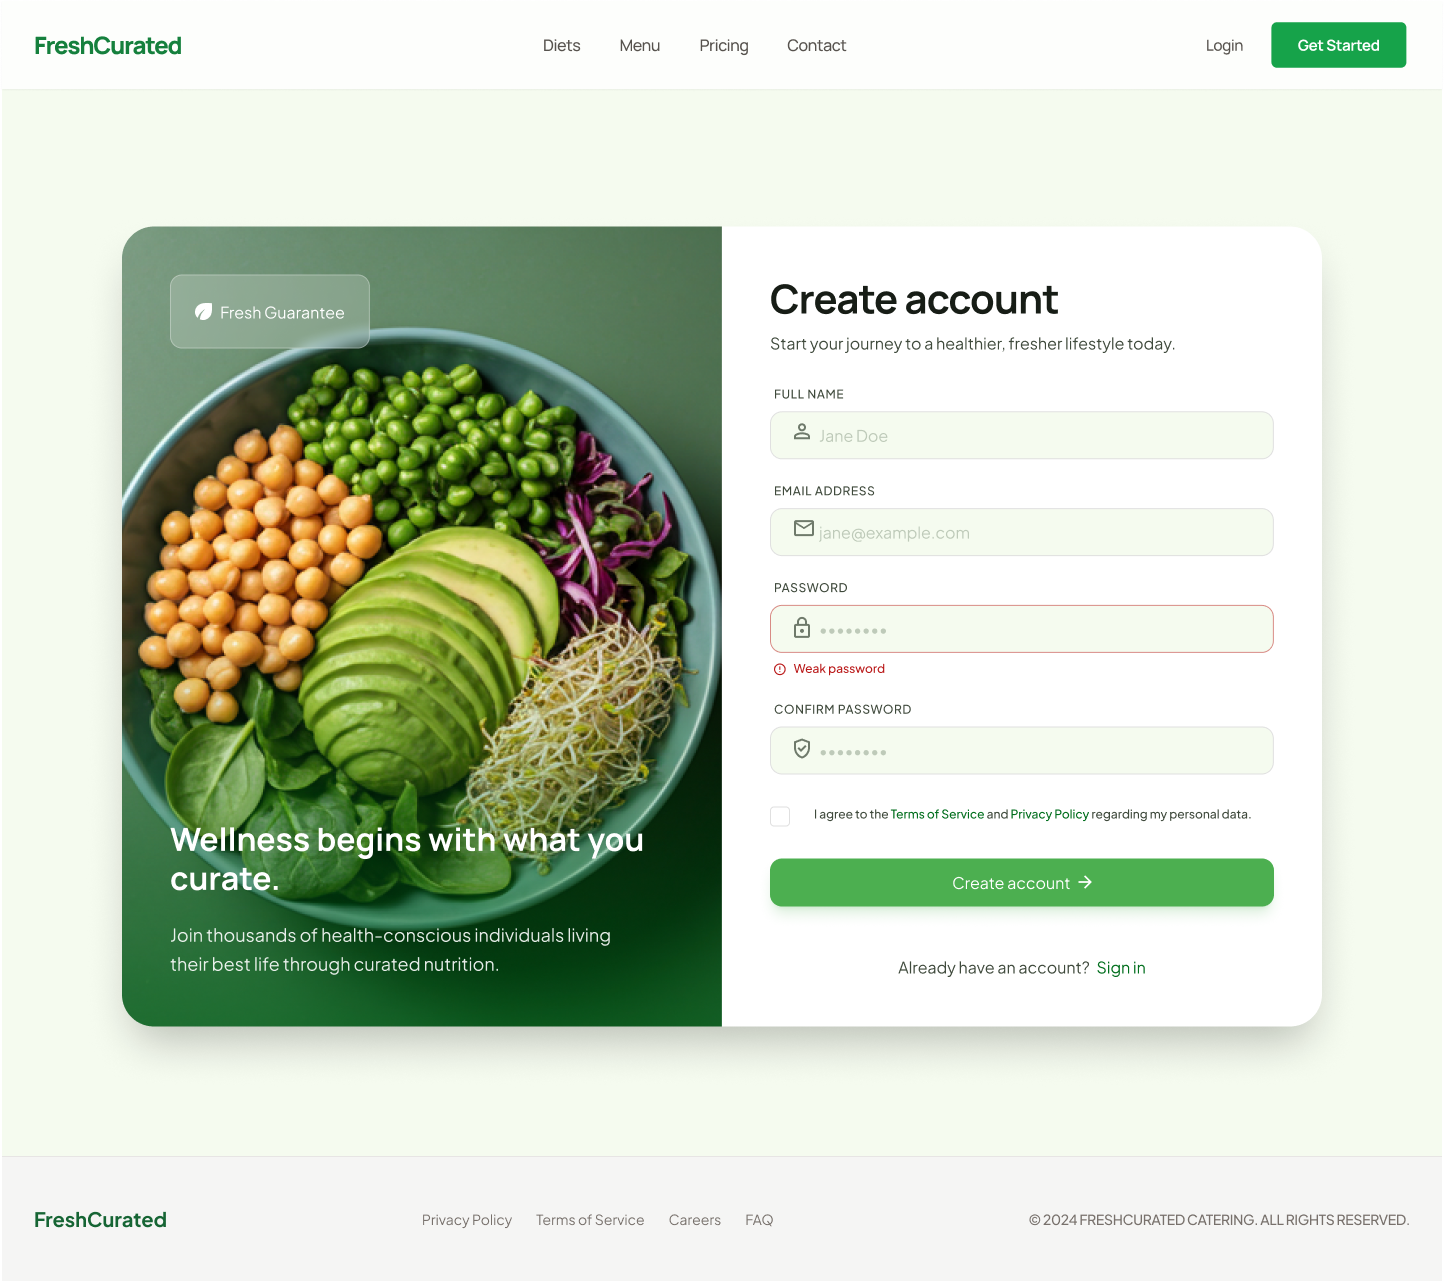
\includegraphics[width=0.6\textwidth]{figures/CreateAccount.png}
    \caption{Ekran tworzenia konta klienta}
    \label{fig:create_account}
\end{figure}

\begin{itemize}
    \item \textbf{Użytkownik niezalogowany}: Głównym celem jest zapoznanie się z ofertą dietetyczną. Funkcjonalności obejmują przeglądanie menu, weryfikację cenników oraz rozpoczęcie procesu składania zamówienia.
    \item \textbf{Użytkownik zalogowany}: Posiada pełny dostęp do personalizacji usług. Funkcjonalności obejmują dostęp do historii zamówień, zarządzanie kontem, edycję adresów dostaw oraz modyfikację parametrów aktywnych diet.
\end{itemize}

\section{Role administracyjne}
Zarządzanie działalnością cateringową podzielono na odrębne kompetencje, co znajduje odzwierciedlenie w strukturze panelu administratora przedstawionego na Rysunku \ref{fig:admin_panel_chapter2}.

\begin{figure}[ht]
    \centering
    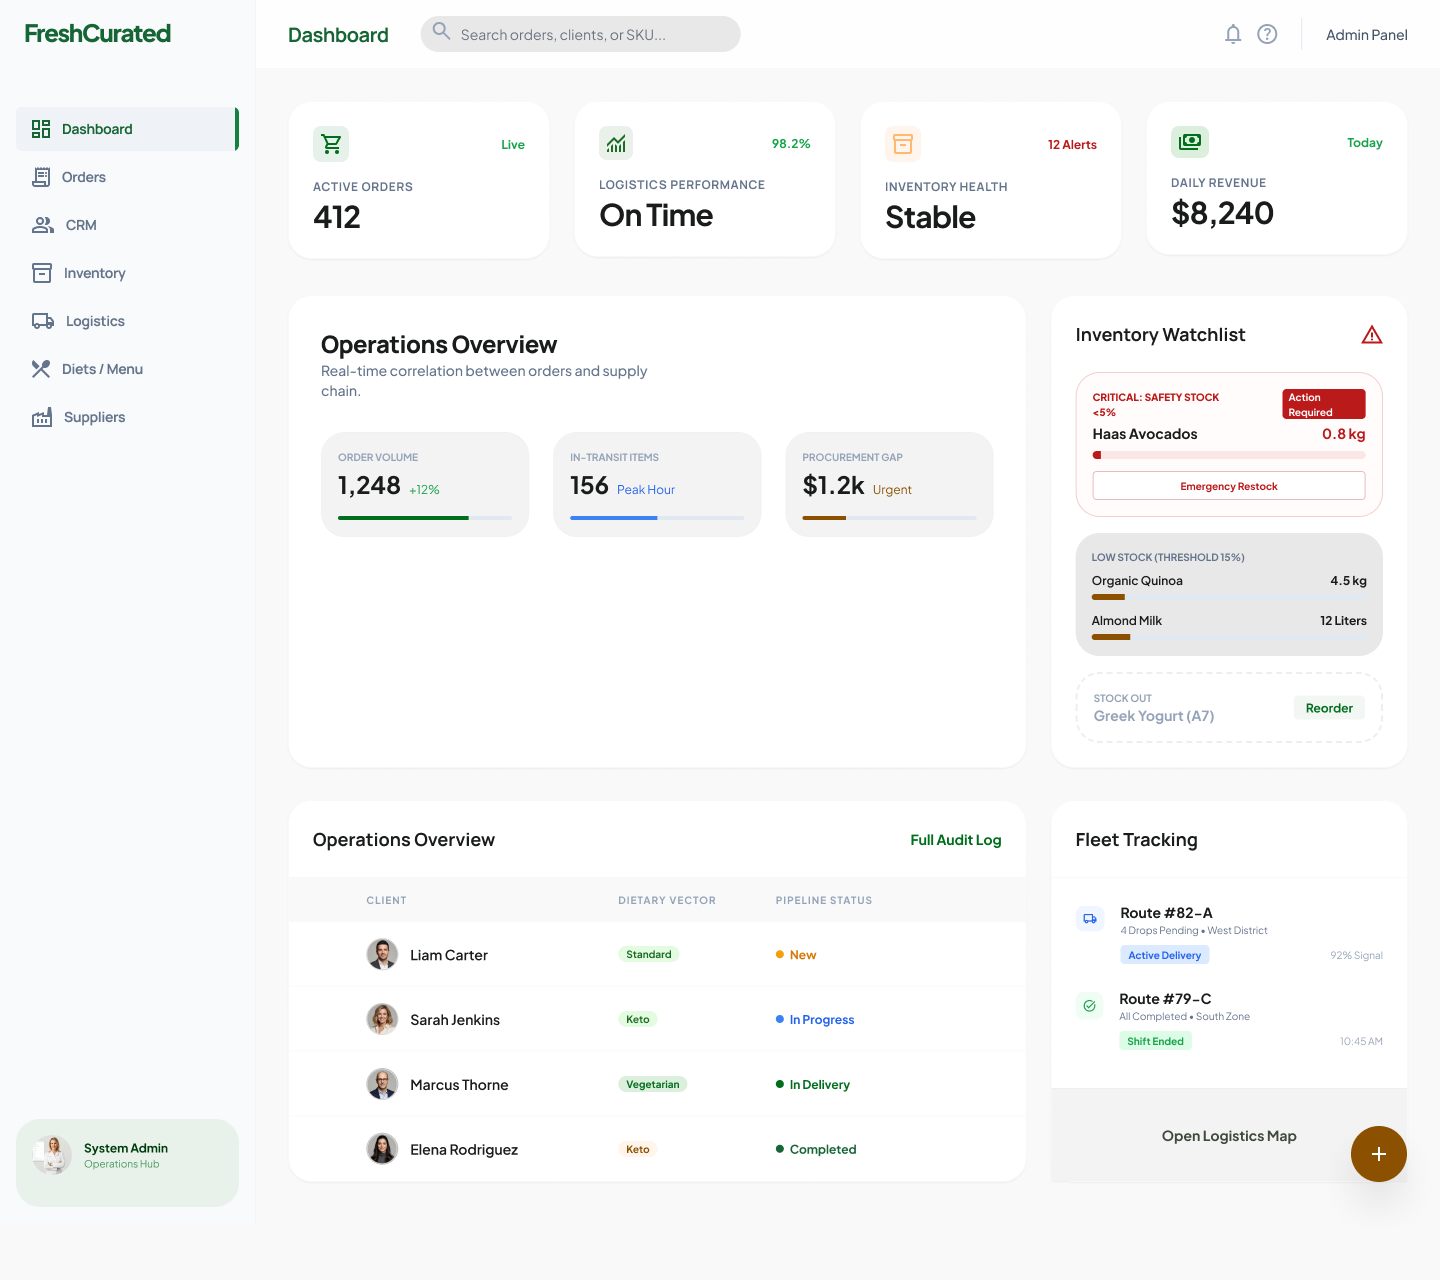
\includegraphics[width=0.8\textwidth]{figures/AdminPanel.png}
    \caption{Panel główny (Dashboard) administratora systemu}
    \label{fig:admin_panel_chapter2}
\end{figure}

Poniższa tabela przedstawia podział odpowiedzialności w zespole administracyjnym:

\begin{table}[ht]
    \centering
    \begin{tabular}{|l|p{8cm}|}
        \hline
        \textbf{Rola} & \textbf{Zakres odpowiedzialności} \\ \hline
        Administrator główny & Pełny dostęp do konfiguracji systemu i raportów. \\ \hline
        Pracownik biura & Bieżąca obsługa zamówień i relacji z klientami. \\ \hline
        Magazynier & Kontrola stanów składników i zarządzanie alertami braków. \\ \hline
        Logistyk/Kurier & Planowanie tras dostaw i nadzór nad realizacją. \\ \hline
    \end{tabular}
    \caption{Podział ról w panelu administracyjnym}
\end{table}

Taka architektura pozwala na bezpieczną separację obowiązków i zwiększa wydajność obsługi procesów biznesowych cateringu.